% -*- mode:latex; mode:flyspell -*-
\documentclass{beamer}[10pt]

% Copyright 2004 by Till Tantau <tantau@users.sourceforge.net>.
%
% In principle, this file can be redistributed and/or modified under
% the terms of the GNU Public License, version 2.
%
% However, this file is supposed to be a template to be modified
% for your own needs. For this reason, if you use this file as a
% template and not specifically distribute it as part of a another
% package/program, I grant the extra permission to freely copy and
% modify this file as you see fit and even to delete this copyright
% notice. 

\mode<presentation> {
  % \usetheme{Warsaw}
  \usetheme{Madrid}
%  \usetheme{Darmstadt}
%  \usetheme{Berkeley}
  % or ...

%  \setbeamercovered{transparent}
  % or whatever (possibly just delete it)
}

\usepackage[english]{babel}
% or whatever

\usepackage[latin1]{inputenc}
% or whatever

\usepackage{hyperref}
\usepackage{cancel}
\usepackage{tikz}
\usetikzlibrary{arrows}
\usetikzlibrary{decorations.markings}
\usetikzlibrary{decorations.pathmorphing}
% \usepackage[absolute,overlay]{textpos}
% \usepackage{onimage}
\usepackage{times}
\usepackage{graphics}
% \usepackage{subfigure}
% \usepackage{scalefnt}
%\usepackage{hyperref}
% \renewcommand\thesubfigure{\arabic{subfigure}}

\graphicspath{{figures}}

% \usepackage{pgfpages}
% \pgfpagesuselayout{2 on 1}[letterpaper,border shrink=2mm,landscape]

% make beamer and subfigure work well
\makeatletter
\def\ext\@subfigure{lof}
\makeatother

% \usepackage{geometry}
% \geometry{letterpaper,landscape}

% \usepackage{caption}
\usepackage[T1]{fontenc}
\usepackage{mathtools}

\usepackage{eso-pic}
%%%%%%%%%%%%%%%%%%%%%%%%%%%%%%%%%%%%%%%%%%%%%%%%%%%%%%%%%%%%%%%%%%%%%%%%%%%%%%%
\usecolortheme{rose}
\definecolor{coolblack}{rgb}{0.0, 0.18, 0.39}
\definecolor{UBCblue}{rgb}{0.0, 0.18, 0.39} % UBC Blue (primary)
\definecolor{UBCgrey}{rgb}{0.3686, 0.5255, 0.6235} % UBC Grey (secondary)
\setbeamercolor{palette primary}{bg=UBCblue,fg=white}
\setbeamercolor{palette secondary}{bg=UBCblue,fg=white}
\setbeamercolor{palette tertiary}{bg=UBCblue,fg=white}
\setbeamercolor{palette quaternary}{bg=UBCblue,fg=white}
\setbeamercolor{structure}{fg=UBCblue} % itemize, enumerate, etc
\setbeamercolor{section in toc}{fg=UBCblue} 
\setbeamertemplate{headline}{}
\setbeamertemplate{itemize items}[circle]
\setbeamertemplate{enumerate items}[default]
%\setbeamertemplate{footline}[frame number]
\setbeamertemplate{frametitle}[default][center]
\setbeamertemplate{navigation symbols}{}
\usefonttheme{serif}
%%%%%%%%%%%%%%%%%%%%%%%%%%%%%%%%%%%%%%%%%%%%%%%%%%%%%%%%%%%%%%%%%%%%%%%%%%%%%%%
% Or whatever. Note that the encoding and the font should match. If T1
% does not look nice, try deleting the line with the fontenc.

\title[VST]{
  {
%  \vspace{-1.0 in}
    {Tracker Meeting: simulation of the first station calibration in a vertical orientation} }
}




% \institute{\inst{1}Univ of Athens, \inst{2}Fermilab , \inst{3}Univ of Glasgow}

\author[Sara Gamba]{
  \fontseries{s}
  \selectfont
  { Sara Gamba, University of Pisa \\ Pavel Murat, FNAL}
}

% \date{\today}
\date{April 29th 2024}
% - Use the \inst command only if there are several affiliations.
% - Keep it simple, no one is interested in your street address.

% - Either use conference name or its abbreviation.
% - Not really informative to the audience, more for people (including
%   yourself) who are reading the slides online


% This is only inserted into the PDF information catalog. Can be left
% out. 

% If you have a file called "university-logo-filename.xxx", where xxx
% is a graphic format that can be processed by latex or pdflatex,
% resp., then you can add a logo as follows:

%%% \pgfdeclareimage[height=0.5cm]{university-logo}{checks\_reorder.png}
%%% \logo{\pgfuseimage{university-logo}}

% Delete this, if you do not want the table of contents to pop up at
% the beginning of each subsection:
%%\AtBeginSubsection[] {
%%%------------------------------------------------------------------------------
%% \begin{frame}<beamer>{\underline{Outline}}
%%    % \tableofcontents[currentsection,currentsubsection]
%%  \tableofcontents[currentsection]
%% \end{frame}
%%}
%%

% If you wish to uncover everything in a step-wise fashion, uncomment
% the following command: 

% \beamerdefaultoverlayspecification{<+->}

\hypersetup{%
  colorlinks=UBCblue,% hyperlinks will be black
  linkbordercolor=UBCblue,% hyperlink borders will be red
  pdfborderstyle={/S/U/W 1}% border style will be underline of width 1pt
}

%%%%%%%%%%%%%%%%%%%%%%%%%%%%%%%%%%%%%%%%%%%%%%%%%%%%%%%%%%%%%%%%%%%%%%%%%%%%%%%
% COMMANDS
%%%%%%%%%%%%%%%%%%%%%%%%%%%%%%%%%%%%%%%%%%%%%%%%%%%%%%%%%%%%%%%%%%%%%%%%%%%%%%%
\newcommand {\baftwo}        {\mbox{$BaF_2$}}
\newcommand {\blue}          {\color{blue}}
\newcommand {\deltaE}        {\mbox{$\delta{\rm-electron}$}}
\newcommand {\eemm}          {\mbox{$ee\mu\mu$}}
\newcommand {\et}            {\mbox{$E_T$}}
\newcommand {\etcorr}        {\mbox{$E_T^{corr}$}}
\newcommand {\gevcsq}        {\mbox{$GeV\!/c^2$}}
\newcommand {\gt}            {\mbox{$>$}}
\newcommand {\invfb}         {\mbox{$fb^{-1}$}}
\newcommand {\invfbrm}       {\mbox{$\rm fb^{-1}$}}
\newcommand {\invpb}         {\mbox{$pb^{-1}$}}
\newcommand {\invpbrm}       {\mbox{$\rm pb^{-1}$}}
\newcommand {\jpsi}          {\mbox{$J/\psi$}}
\newcommand {\lt}            {\mbox{$<$}}
\newcommand {\met}           {\mbox{${\not\! E}_{T}$}}
\newcommand {\mmmm}          {\mbox{$\mu\mu\mu\mu$}}
\newcommand {\mzz}           {\mbox{$M_{ZZ}$}}
\newcommand {\pb}            {\mbox{\rm\,pb}}
\newcommand {\ppbar}         {\mbox{$p\bar{p}$}}
\newcommand {\pt}            {\mbox{$p_T$}}
\newcommand {\red}           {\color{red}}
\newcommand {\stat}          {\mbox{\rm (stat.)}}
\newcommand {\statsys}       {\mbox{\rm (stat.+syst.)}}
\newcommand {\syst}          {\mbox{\rm (syst.)}}
\newcommand {\wpigamma}      {\mbox{$W^{\pm} \rightarrow \pi^{\pm} \gamma$}}
\newcommand {\wenu}          {\mbox{$W^{\pm} \rightarrow e^{\pm} \nu$}}
\newcommand {\wlnu}          {\mbox{$W^{\pm} \rightarrow l^{\pm} \nu$}}
\newcommand {\wmunu}         {\mbox{$W^{\pm} \rightarrow \mu^{\pm} \nu$}}
\newcommand {\wtaunu}        {\mbox{$W^{\pm} \rightarrow \tau^{\pm} \nu$}}
\newcommand {\zpsigamma}     {\mbox{$    Z^{0} \rightarrow J/\psi \gamma$}}
\newcommand {\zpigamma}      {\mbox{$\rm Z^{0} \rightarrow \pi^{0} \gamma$}}
\newcommand {\zee}           {\mbox{$\rm Z^0 \rightarrow e^+ e^-$}}
\newcommand {\zmumu}         {\mbox{$\rm Z^0 \rightarrow \mu^+ \mu^-$}}
\newcommand {\ztautau}       {\mbox{$\rm Z^0 \rightarrow \tau^+ \tau^-$}}
\newcommand {\zll }          {\mbox{$Z       \rightarrow l^{+}l^{-}$}}
\newcommand {\zupsgamma}     {\mbox{$    Z^0 \rightarrow \Upsilon \gamma$}}
\newcommand {\zzx }          {\mbox{$X       \to ZZ$}}
\newcommand {\zzllll}        {\mbox{$ZZ \to \ell^+ \ell^- \ell^+ \ell^-$}}
\newcommand {\zzllnn}        {\mbox{$ZZ \to \ell^+ \ell^- \nu \nu$}}
\newcommand {\zzlljj}        {\mbox{$ZZ \to \ell^+ \ell^- j j$}}

%\newcommand {\plots}  {/home/murat/figures}   % MURAT03

   % MURAT05
% \newcommand {\plots}  {/home/murat/figures/drs4}   % MURAT03


\begin{document}

%------------------------------------------------------------------------------
% working document - no title page
%------------------------------------------------------------------------------
% \begin{frame}
%   \titlepage
% \end{frame}
% -------------------------------------- uncomment this to get the table of contents 
% \begin{frame}{\underline{Outline}}
% \tableofcontents % [pausesections]
%  % You might wish to add the option [pausesections]
% \end{frame}
% 
%------------------------------------------------------------------------------
% \AtBeginSection[] {
%    \begin{frame}<beamer>{}
     %     \tableofcontents[currentsection,currentsubsection]
%    \tableofcontents[currentsection]
%    \end{frame}
% }
% 
% Structuring a talk is a difficult task and the following structure
% may not be suitable. Here are some rules that apply for this
% solution: 

% - Exactly two or three sections (other than the summary).
% - At *most* three subsections per section.
% - Talk about 30s to 2min per frame. So there should be between about
%   15 and 30 frames, all told.

% - A conference audience is likely to know very little of what you
%   are going to talk about. So *simplify*!
% - In a 20min talk, getting the main ideas across is hard
%   enough. Leave out details, even if it means being less precise than
%   you think necessary.
% - If you omit details that are vital to the proof/implementation,
%   just say so once. Everybody will be happy with that.
%%%%%%%%%%%%%%%%%%%%%%%%%%%%%%%%%%%%%%%%%%%%%%%%%%%%%%%%%%%%%%%%%%%%%%%%%%%%%%%

\begin{frame}
\centering
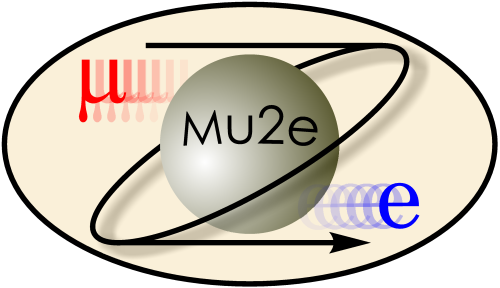
\includegraphics[height=1cm]{figures/png/mu2e_logo_oval.png}
\titlepage
\centering

\includegraphics[height=0.9cm]{figures/png/FNAL-Logo-NAL-Blue.png}\hspace{10mm}
\includegraphics[height=1.6cm]{figures/pdf/cherubino.pdf}

\end{frame}
\begin{frame}{Introduction: VST and calibration}
  \begin{itemize}
  \item The first station is expected soon;
  \vspace{1mm}
  \item Reconstructing cosmic tracks and understanding resolutions requires calibrating the station.
  \end{itemize}
  \vspace{3mm}
 Timing calibration:
 \vspace{1mm}
  \begin{itemize}
    \item signal propagation and channel-to-channel delays for each straw.
  \end{itemize}
  \vspace{3mm}
  What is it needed for this purpose?
  \vspace{1mm}
  \begin{itemize}
    \item unbiased reconstruction of the track longitudinal position in a straw.
  \end{itemize}
 
\end{frame}


\begin{frame}{Introduction: station orientation}
  
  During CM, there was a discussion related to the orientation of the station:
  \vspace{1mm}
  \begin{itemize}
    \item Vertical orientation is preferred for gas system and because the station will be vertical during the experiment;
    \vspace{1mm}
  \item Horizontal orientation enables an unbiased reconstruction. First VST plane calibration was horizonal.
\end{itemize}
\vspace{3mm}
Would running in vertical orientation provide data needed for calibrating?
\vspace{3mm}
\\
A simulation has been performed to reconstruct cosmics tracks with vertically oriented station,
  aiming to understand possible biases in determining longitudinal position caused by the non-uniform illumination of a panel.
\end{frame}

\begin{frame}{Reconstruction of Cosmic tracks}
  \begin{columns}
    \begin{column}{0.6 \framewidth}
      \begin{itemize}
  \item The station is not yet calibrated: whether a straw has been hit or not is the only info we have;
  \vspace{3mm}
\item 4 hits per face to reconstruct one line:
        \begin{itemize}
          \item panel hits in each face $\rightarrow$ combo hits;
          \item 2 combo hits in a plane $\rightarrow$ stereo hit;
          \item 2 hits per plane $\rightarrow$ reconstructed track.
        \end{itemize}
        \vspace{3mm}

  \item The reconstruction of the hit position is performed using:
  \vspace{2mm}

    \begin{itemize}
        \item the straw direction  $(D_x,D_y)$;
        \vspace{1mm}
        \item the straw midpoints $(x,y)$;
        \vspace{1mm}
        \item the straw $z$ coordinate of faces.
    \end{itemize} 
  \end{itemize} 
  \end{column}
  \begin{column}{0.4 \framewidth}
    \begin{figure}[H]
      \centering
      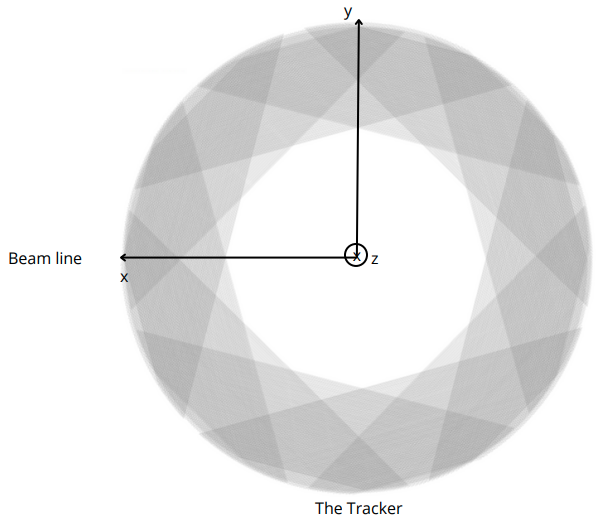
\includegraphics[width=0.8 \columnwidth]{figures/png/Screenshot_20240408_154724.png}
      \label{fig:enter-label}
  \end{figure}
  \end{column}

  \end{columns}
  \end{frame}


\begin{frame}{Cosmics simulation and selection criteria}
  \begin{itemize}
    \item Simulated cosmics crossing only one station;
    \vspace{3mm}
    \item Station in vertical orientation in extracted position;
    \vspace{3mm}
    \item No magnetic field;
    \vspace{3mm}
    \item To reconstruct a straight line in 3D, at least 4 hits at different $z$ are needed: tracks selected with $nhits_{face_i}\geq 1$;
    \vspace{3mm}
    \item To improve the resolution, $nhits_{panel_i}\leq 3$ were selected.
  \end{itemize}
\end{frame}



\begin{frame}{Panel illumination}
   \vspace{-3mm}
            \begin{figure}[H]
                \centering
                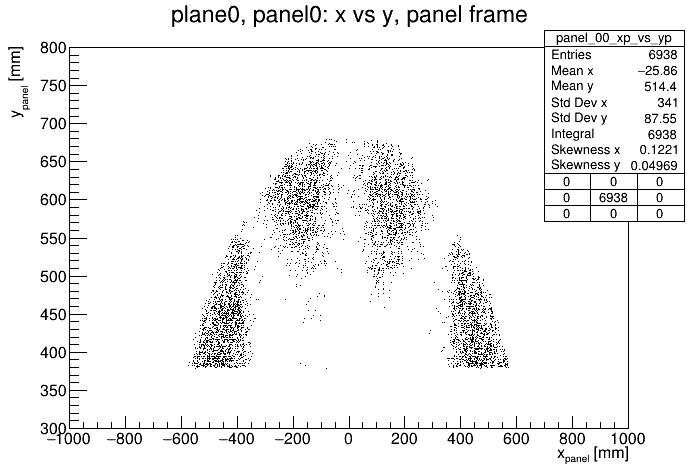
\includegraphics[width=0.7 \textwidth]{figures/pdf/xp_vs_yp_panel0.png}
                \label{fig:enter-label}
            \end{figure}
\begin{itemize}
  \item spotty and non uniform illumination pattern of a panel in a vertical orientation (panel frame);
    \item same for all panels;
  \item wires have no hits in the center.
\end{itemize}

\end{frame}





\begin{frame}{Results: longitudinal position reconstruction}
  \vspace{-3mm}
  \begin{columns}
    \begin{column}{0.5\framewidth}
      \begin{figure}[H]
        \centering
        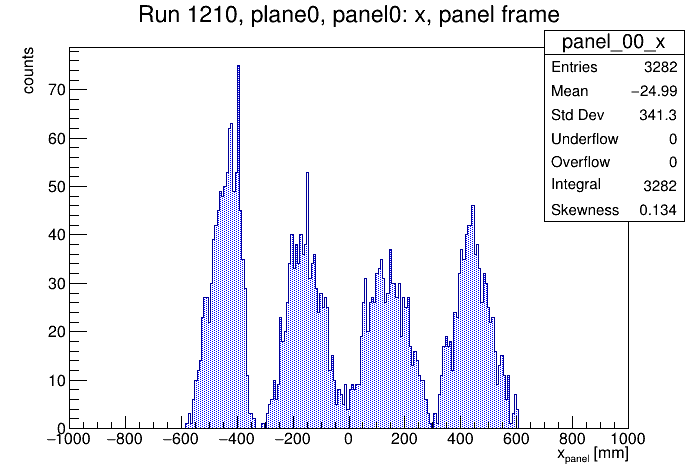
\includegraphics[width= \textwidth]{figures/pdf/x_panel0.png}
        \label{fig:enter-label}
    \end{figure}
    \vspace{-12mm}
    \begin{figure}[H]
      \centering
      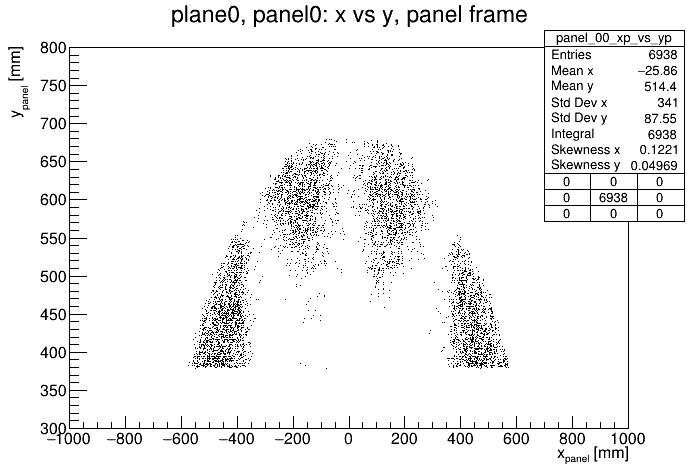
\includegraphics[width=  \textwidth]{figures/pdf/xp_vs_yp_panel0.png}
      \label{fig:enter-label}
  \end{figure}
     
    \end{column}
    \begin{column}{0.5\framewidth}
      \begin{itemize}
        \item the histogram shows longitudinal position in the panel frame;
        \vspace{3mm}
      \item reconstructed longitudinal position distribution presents peaks in the overlaps with other panels;
        \vspace{3mm}
      \item different straws make different peaks.
      \end{itemize}
    \end{column}
  \end{columns}
\end{frame}




\begin{frame}{Results: longitudinal position reconstruction bias}
  \vspace{-3mm}
  \begin{columns}
    \begin{column}{0.5\framewidth}
      \begin{figure}[H]
        \centering
        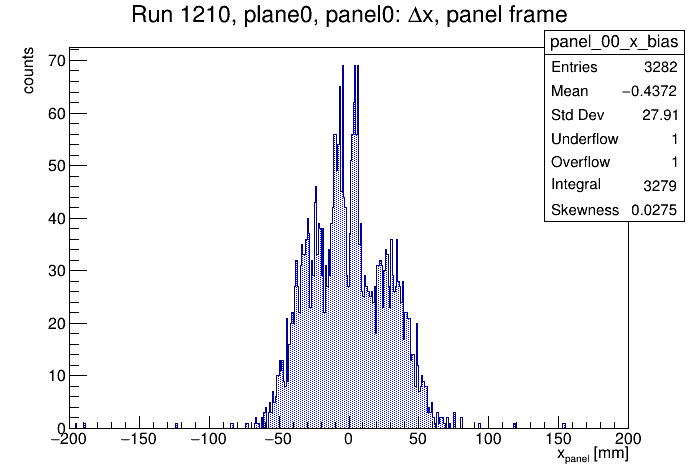
\includegraphics[width= \textwidth]{figures/pdf/panel_00_x_bias.png}
        \label{fig:enter-label}
    \end{figure}
    \vspace{-12mm}
    \begin{figure}[H]
      \centering
      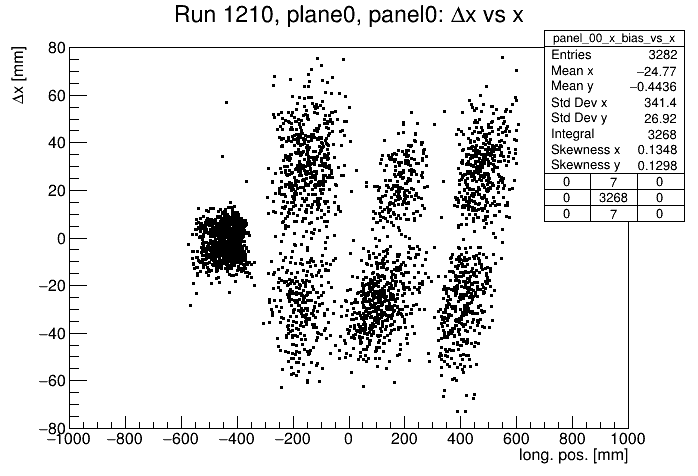
\includegraphics[width=  \textwidth]{figures/pdf/panel_00_x_bias_vs_x.png}
      \label{fig:enter-label}
  \end{figure}
     
    \end{column}
    \begin{column}{0.5\framewidth}
      \begin{itemize}
       
      \item reconstructed longitudinal position distribution presents peaks in the overlaps with other panels;
        \vspace{3mm}
      \item $\Delta x = x_{rec}-x_{true}$;
      \vspace{3mm}
        \item the longitudinal position bias range is about -6$\div$6 cm;
        \vspace{3mm}
        \item 2D distribution of $\Delta x$ versus $x_{true}$ shows four different spots referring to the overlap regions;
        \vspace{3mm}
        \item the first spot (CAL side) is referred to ninety degrees panels overlap.
      \end{itemize}
    \end{column}
  \end{columns}
\end{frame}


\begin{frame}{Results: systematics on longitudinal position reconstruction}

   
    \begin{figure}[H]
      \centering
      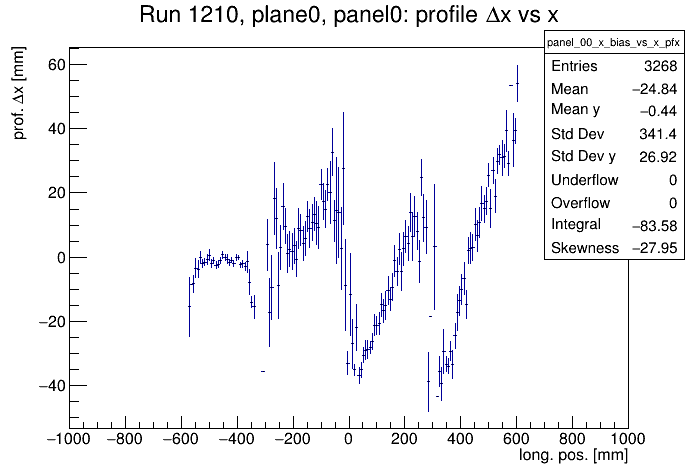
\includegraphics[width= 0.5\textwidth]{figures/pdf/panel_00_x_bias_vs_x_prof.png}
      \label{fig:enter-label}
  \end{figure}
   
      \begin{itemize}
      
        
        \item  profile of the $\Delta x$ versus $x_{true}$ shows a systematic effect in determining the longitudinal position of a range greater than -4$\div$4 cm;
        \vspace{3mm}
        \item the first part (CAL side) is referred to ninety degrees panels overlap;
        \vspace{3mm}
        \item the mean is not a good estimator of the bias, because the distribution is referred to multiple straws.
      \end{itemize}

  
\end{frame}

\begin{frame}{Direction of the reconstructed line}
  \vspace{-3mm}

  \begin{columns}
    \begin{column}{0.5\framewidth}
  \begin{figure}[H]
    \centering
    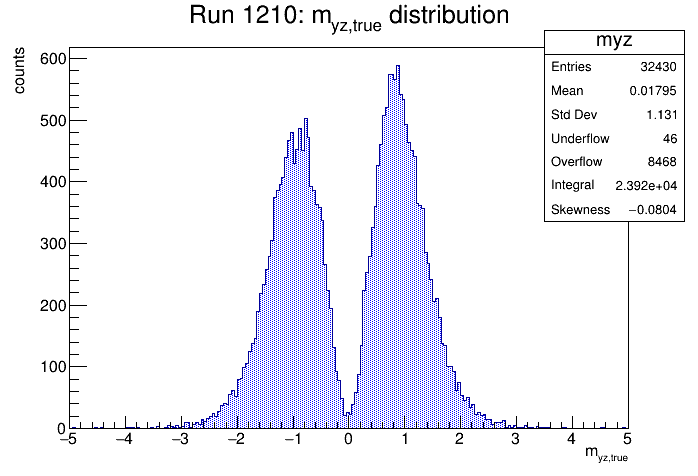
\includegraphics[width= \textwidth]{figures/pdf/myz.png}
    \label{fig:enter-label}
\end{figure}
\vspace{-12mm}
\begin{figure}[H]
  \centering
  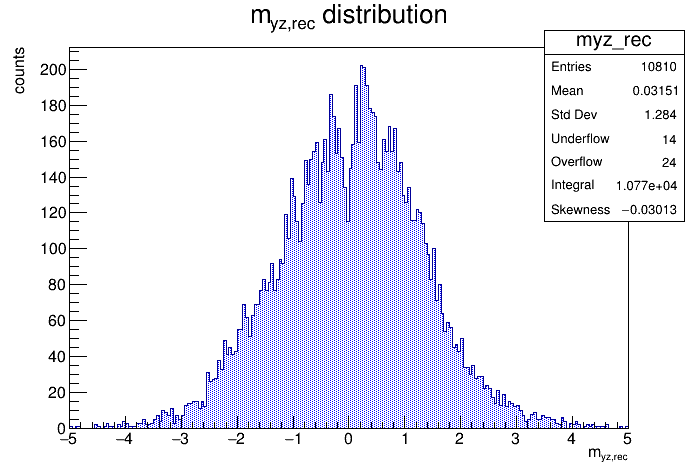
\includegraphics[width= \textwidth]{figures/pdf/myz_rec.png}
  \label{fig:enter-label}
\end{figure}

\end{column}
\begin{column}{0.5\framewidth}

  \begin{itemize}
      
    \item $m_{yz}=\frac{\Delta y}{\Delta z}$;
    \vspace{2mm}
    \item first histogram shows true $m_{yz}$;
    \vspace{2mm}
    \item second histogram shows the reconstructed $m_{yz}$;
    \vspace{2mm}
    \item true hits position far away from the straws midpoint lead to the misreconstructed $zy$ and $xy$ direction lines.
  \end{itemize}
\end{column}
\end{columns}
\end{frame}


\begin{frame}{Conclusions}
  In a vertical configuration of the station:
  \vspace{6mm}
  \begin{itemize}
    \item illumination of panels is very non uniform, no hits in the central part of wires;
    \vspace{4mm}
    \item there will be systematic effects in determining the longitudinal position ($\sim$ cm) due to the panel orientation;
    \vspace{4mm}
    \item calibration is expected to be very difficult in these conditions.
  \end{itemize}
\end{frame}




\begin{frame}{Backup Slide: Combo, Stereo Hits and Reconstructed line}
  \vspace{-3mm}
\begin{columns}
\begin{column}{0.5\framewidth}
  \vspace{-15mm}

  $$\textbf{\text{1. Geometrical Combo Hits}}$$
  Determination of a unique straw in a panel:
  \begin{itemize}
    \item mean of straws midpoint $(x_m,y_m,z_m)$;
    \item straws direction $(D_x,D_y)$.
  \end{itemize}
\end{column}
\begin{column}{0.5\framewidth}
  $$\textbf{\text{2. Geometrical Stereo Hits}}$$
  Determination of the hit point in a plane:
  \begin{itemize}
    \item intersection point $(x,y)$ using the two straws directions and midpoints from two panels;
    \item mean of $z$ coordinate between the two faces.
  \end{itemize}
\end{column}
\end{columns}
\vspace{5mm}

$$\textbf{\text{3. Reconstructed Line}}$$
Determination of a unique reconstructed track:
\begin{itemize}
\item one stereo hit per plane: one line reconstructed geometrically;
\item the intersection point of the line with panels is found knowing the $z_m$ coordinate. 
\end{itemize}

\end{frame}



\begin{frame}{Backup Slide}
  
      \begin{figure}[H]
        \centering
        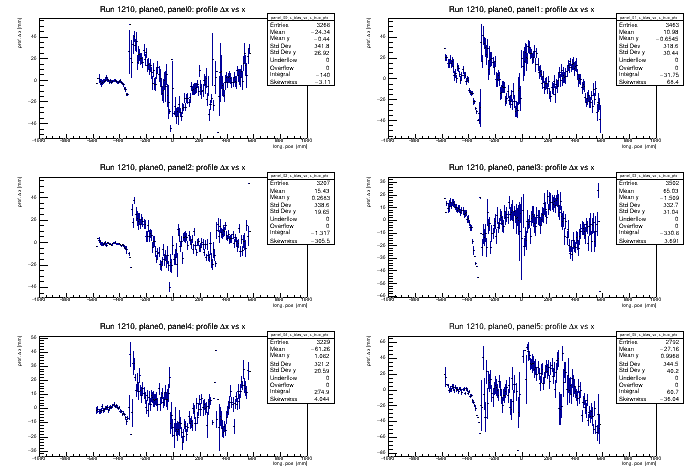
\includegraphics[width= \textwidth]{figures/pdf/plane0_prof_bias.png}
        \label{fig:enter-label}
    \end{figure}
  \end{frame}

  \begin{frame}{Backup Slide}
    \vspace{-3mm}

    \begin{columns}
      \begin{column}{0.5\framewidth}
    \begin{figure}[H]
      \centering
      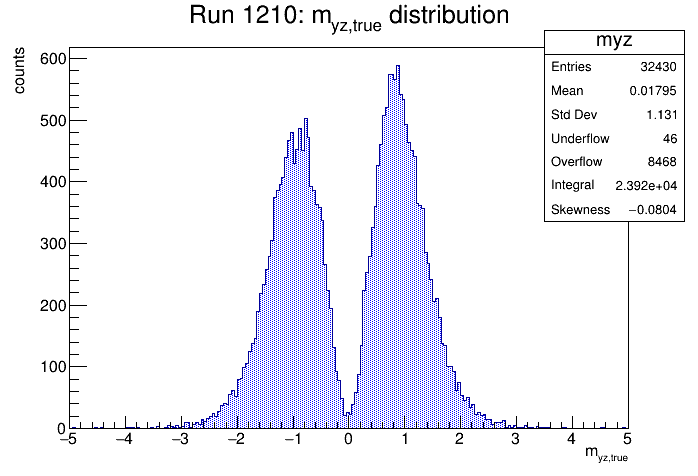
\includegraphics[width= \textwidth]{figures/pdf/myz.png}
      \label{fig:enter-label}
  \end{figure}
  \vspace{-12mm}

  \begin{figure}[H]
    \centering
    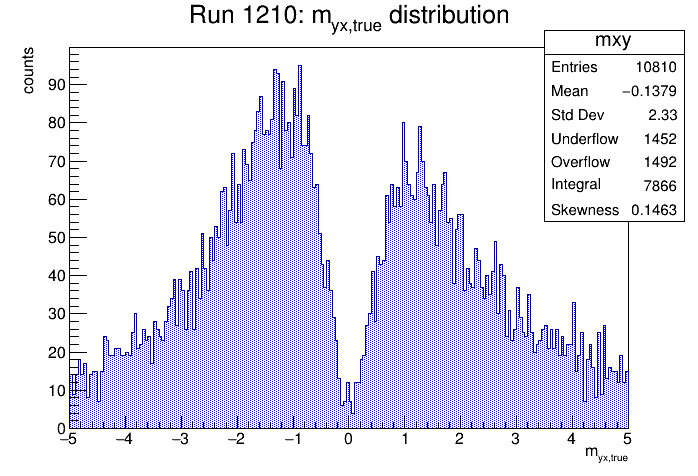
\includegraphics[width= \textwidth]{figures/pdf/mxy.png}
    \label{fig:enter-label}
\end{figure}
\end{column}
\begin{column}{0.5\framewidth}
  \begin{figure}[H]
    \centering
    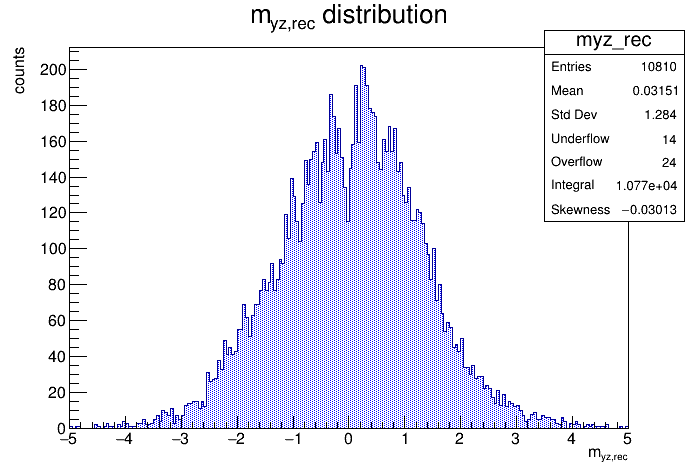
\includegraphics[width= \textwidth]{figures/pdf/myz_rec.png}
    \label{fig:enter-label}
\end{figure}
\vspace{-12mm}

\begin{figure}[H]
  \centering
  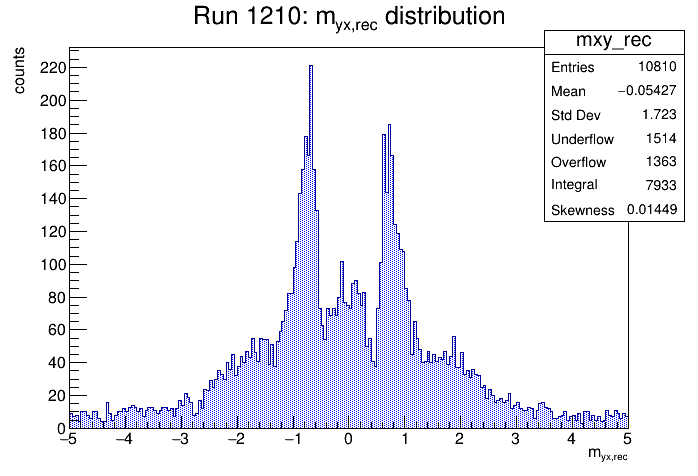
\includegraphics[width= \textwidth]{figures/pdf/mxy_rec.png}
  \label{fig:enter-label}
\end{figure}
\end{column}
\end{columns}
\end{frame}
\begin{frame}{Results: systematics on track direction reconstruction}
  \vspace{-3mm}
  \begin{columns}
    \begin{column}{0.5\framewidth}
      \begin{figure}[H]
        \centering
        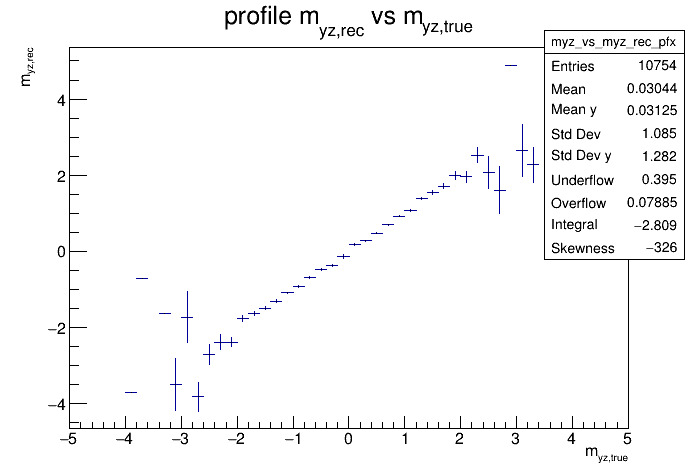
\includegraphics[width= \textwidth]{figures/pdf/myz_vs_myz_rec_prof.png}
        \label{fig:enter-label}
    \end{figure}
     
    \vspace{-12mm}
    \begin{figure}[H]
      \centering
      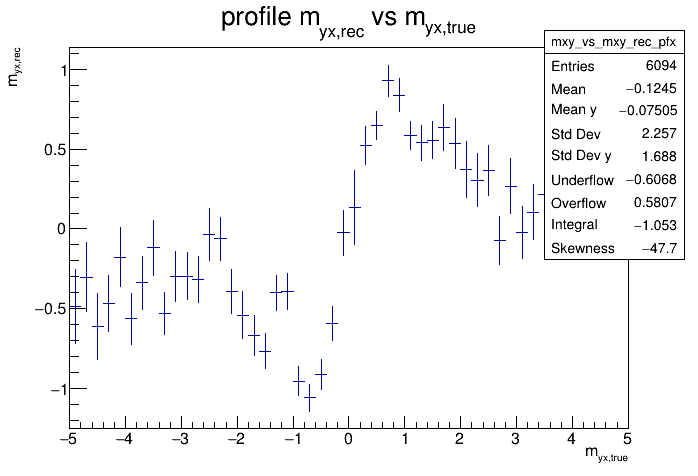
\includegraphics[width= \textwidth]{figures/pdf/myx_vs_myx_rec_prof.png}
      \label{fig:enter-label}
  \end{figure}
    \end{column}
    \begin{column}{0.5\framewidth}
      \vspace{-4mm}

      \begin{itemize}
        \item $m_{yz}=\frac{\Delta y}{\Delta z}$ and $m_{yx}=\frac{\Delta y}{\Delta x}$;
        \vspace{2mm}
        \item first histogram shows the mean of reconstructed $m_{yz}$ versus the true one and it shows a systematic effect in determining the $zy$ track direction (-4$\div$3);
        \vspace{2mm}
        \item second histogram shows the mean of reconstructed $m_{yx}$ versus the true one and it shows a systematic effect in determining the $xy$ track direction (-1$\div$1);
        \vspace{2mm}
        \item true hits position far away from the straws midpoint lead to the misreconstructed $zy$ and $xy$ direction lines.
      \end{itemize}
    \end{column}
  \end{columns}
\end{frame}

\end{document}
